\chapter{Keyboard Driver}\label{chapter:Keyboard Driver}

\section{Writing and reading from ports}\label{section:Writing and reading from ports}

Before writing a device driver, the functionality to communicate with different I/O ports needs to be implemented.
This is done in assembly using the \textbf{outb} and \textbf{inb} instructions.
The code can be written using extended asm:

\begin{lstlisting}
    // Read a byte from port
    inline unsigned char inportb(unsigned int port)
    {
        unsigned char ret;
        asm volatile("inb %%dx,%%al"
                    : "=a"(ret)
                    : "d"(port));
        return ret;
    }

    // Write value to port
    inline void outportb(unsigned int port, unsigned int value)
    {
        asm volatile("outb %%al,%%dx"
                    :
                    : "d"(port), "a"(value));
    }
\end{lstlisting}

\section{Overview}\label{Overview}

When the user presses a key, an interrupt is raised which causes the keyboard ISR to be called.\\
This ISR instructs the keyboard driver to read the character from the keyboard port. This character is then
printed to the screen and saved in a circular buffer. During scanf(), this input is read from the circular buffer.

\section{Understanding Keyboard ports}\label{section:Understanding Keyboard ports}
The PS/2 keyboard uses two main ports:
\begin{itemize}
    \item \textbf{0x60} - This is the data port from which characters are read.
    \item \textbf{0x64} - This is the command port to which commands are issued.\\
     Reading from this port gives status information.
\end{itemize}

\begin{figure}[h!]
    \begin{center}
        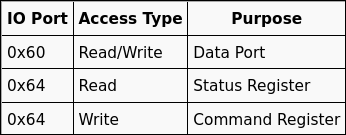
\includegraphics[width=200px,height=200px,keepaspectratio]{kbd_port}
        \caption{Summary of keyboard ports}
    \end{center}
\end{figure}

\begin{figure}[h!]
    \begin{center}
        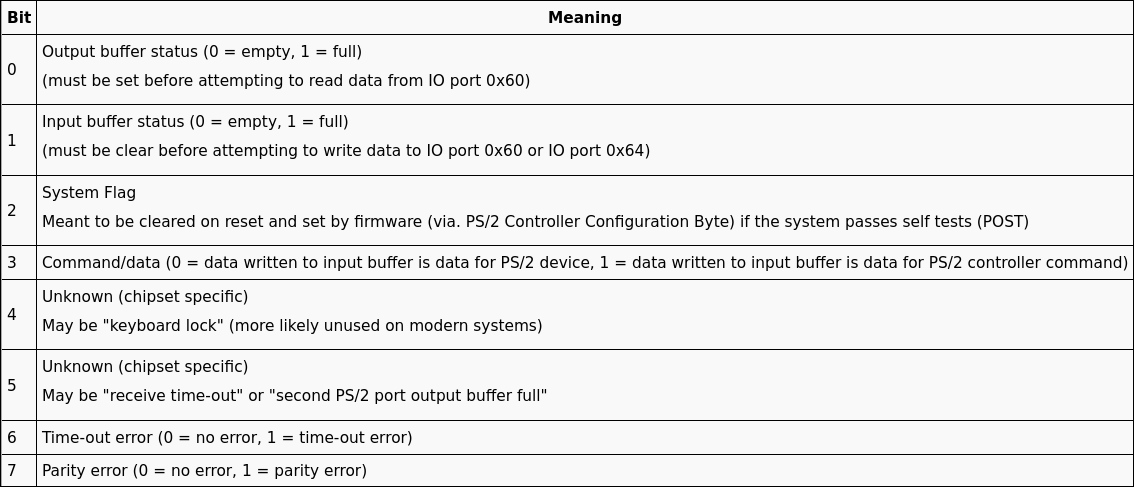
\includegraphics[width=350px, height=350px,keepaspectratio]{kbd_status}
        \caption{Keyboard Status}
    \end{center}
\end{figure}

\pagebreak
\section{Scan code to character conversion}\label{section:Scan code to character conversion}
The data read from the keyboard data port is not an ASCII representation of the character associated with a key press.
Instead the data is a scan code which must further be converted to an ASCII character.
There are three scan code sets that are used by keyboards. 
DaxOS uses scan code set one. 

\vspace{0.5cm}
As an example consider that a user presses the `A' key on the keyboard. The data from the keyboard will be 0x1E which corresponds to
`A' on scan code set 1.

\vspace{0.5cm}
DaxOS does this conversion using a lookup table in \textbf{kbd\_table.h}.

\begin{lstlisting}
    static const char kbd_scan_tbl[236] = {
        '\0','\0','1','2','3','4','5','6','7','8','9',
        '0','\0','\0','\b','\0','q','w','e','r','t',
        'y','u','i','o','p','\0','\0','\n','\0','a',
        's','d','f','g','h','j','k','l','\0','\0',
        '\0','\0','\0','z','x','c','v','b','n','m',
        ...
    };
\end{lstlisting}

The `\textbackslash0' here are for characters that are ignored.

\section{Keyboard Driver API}\label{section:Keyboard Driver API}

The keyboard driver API is as follows:
\begin{lstlisting}
    uint8_t kbd_read_status();
    uint8_t kbd_read_data();
    void kbd_data_send_cmd(uint8_t cmd);
    void kbd_ack();
    void kbd_ctrl_send_cmd(uint8_t cmd);
    void kbd_enable_interrupts();
\end{lstlisting}